% (The MIT License)
%
% Copyright (c) 2023-2024 Yegor Bugayenko
%
% Permission is hereby granted, free of charge, to any person obtaining a copy
% of this software and associated documentation files (the 'Software'), to deal
% in the Software without restriction, including without limitation the rights
% to use, copy, modify, merge, publish, distribute, sublicense, and/or sell
% copies of the Software, and to permit persons to whom the Software is
% furnished to do so, subject to the following conditions:
%
% The above copyright notice and this permission notice shall be included in all
% copies or substantial portions of the Software.
%
% THE SOFTWARE IS PROVIDED 'AS IS', WITHOUT WARRANTY OF ANY KIND, EXPRESS OR
% IMPLIED, INCLUDING BUT NOT LIMITED TO THE WARRANTIES OF MERCHANTABILITY,
% FITNESS FOR A PARTICULAR PURPOSE AND NONINFRINGEMENT. IN NO EVENT SHALL THE
% AUTHORS OR COPYRIGHT HOLDERS BE LIABLE FOR ANY CLAIM, DAMAGES OR OTHER
% LIABILITY, WHETHER IN AN ACTION OF CONTRACT, TORT OR OTHERWISE, ARISING FROM,
% OUT OF OR IN CONNECTION WITH THE SOFTWARE OR THE USE OR OTHER DEALINGS IN THE
% SOFTWARE.

\documentclass{article}
\usepackage{setspace}
\usepackage[static]{/code/ctan/clicks/clicks}
\usepackage{../lecture-notes/notes}
\newcommand*\thetitle{Code Churn}
\begin{document}

\plush{\lnTitlePage{13}{24}{dvuyJ5LvHvQ}}

\lnPitch{
  \pptBanner{History of Version Control Systems (VCS)}
  \begin{itemize}\setlength\itemsep{-.2em}
    \item The \textbf{Librarian} by ADR: created in 1969
    \item \textbf{Panvalet} by Computer Associates: 1969
    \item \textbf{SCCS} by Bell Labs: 1973
    \item \textbf{RCS} by GNU: 1982
    \item \textbf{CVS} by Dick Grune: 1986
    \item \textbf{ClearCase} by IBM: 1992
    \item \textbf{Subversion} by Apache: 2000
    \item \textbf{BitKeeper} by BitMover Inc.: 2000
    \item \textbf{Arch} by Thomas Lord in GNU: 2001
    \item \textbf{Git} by Linus Torvalds: 2005
    \item \textbf{Mercurial} by Olivia Mackall: 2005
  \end{itemize}}

\lnQuote
  [Sebastian G. Elbaum]
  {sebastian-elbaum}
  {We can measure the increase or decrease in system complexity as measured by a selected metric, \ul{code delta}, or we can measure the total amount of \ul{change} the system has undergone between builds, \textcolor{orange}{code churn}.}
  {munson1998}

\lnPitch{
  \pptBanner{What is ``Churn''?}
  \begin{multicols}{2}
  Wikipedia says that ``\textcolor{orange}{churn rate}
  (also known as attrition rate, turnover, customer turnover, or
  customer defection) is a measure of the proportion of individuals or
  items \ul{moving out} of a group over a specific period.''
  \par\columnbreak\par
  \pptPic{1}{butter-churn.jpg}\par
  {\small Barrel Butter Churn, Victorian, Original, \$95.00\par}
  \end{multicols}}

\pptBanner{Motivating Example}
\begin{pptWide}{3}
Commit \#1:\par
0\par
{\small\begin{ffcode}
class Book
  private final int id;
  public Book(int it)
    this.id = i;
\end{ffcode}
}
\par\columnbreak\par
Commit \#2:\par
\textcolor{green}{+5}\par
{\small\begin{ffcode}
class Book
  private int id;
  public Book(int it)
    this.id = i;
  public int getId()
    return this.id;
  private int setId(int i)
    this.id = i;
\end{ffcode}
}
\par\columnbreak\par
Commit \#3:\par
\textcolor{green}{+2} / \textcolor{red}{-2}\par
{\small\begin{ffcode}
final class Book
  private final int id;
  public Book(int it)
    this.id = i;
  public int getId()
    return this.id;
\end{ffcode}
}
\end{pptWide}
Delta: \textcolor{green}{+3} / 0, Churn: \textcolor{green}{+7} / \textcolor{red}{-2}
\plush{}

\lnPitch{
  \begin{multicols}{2}
  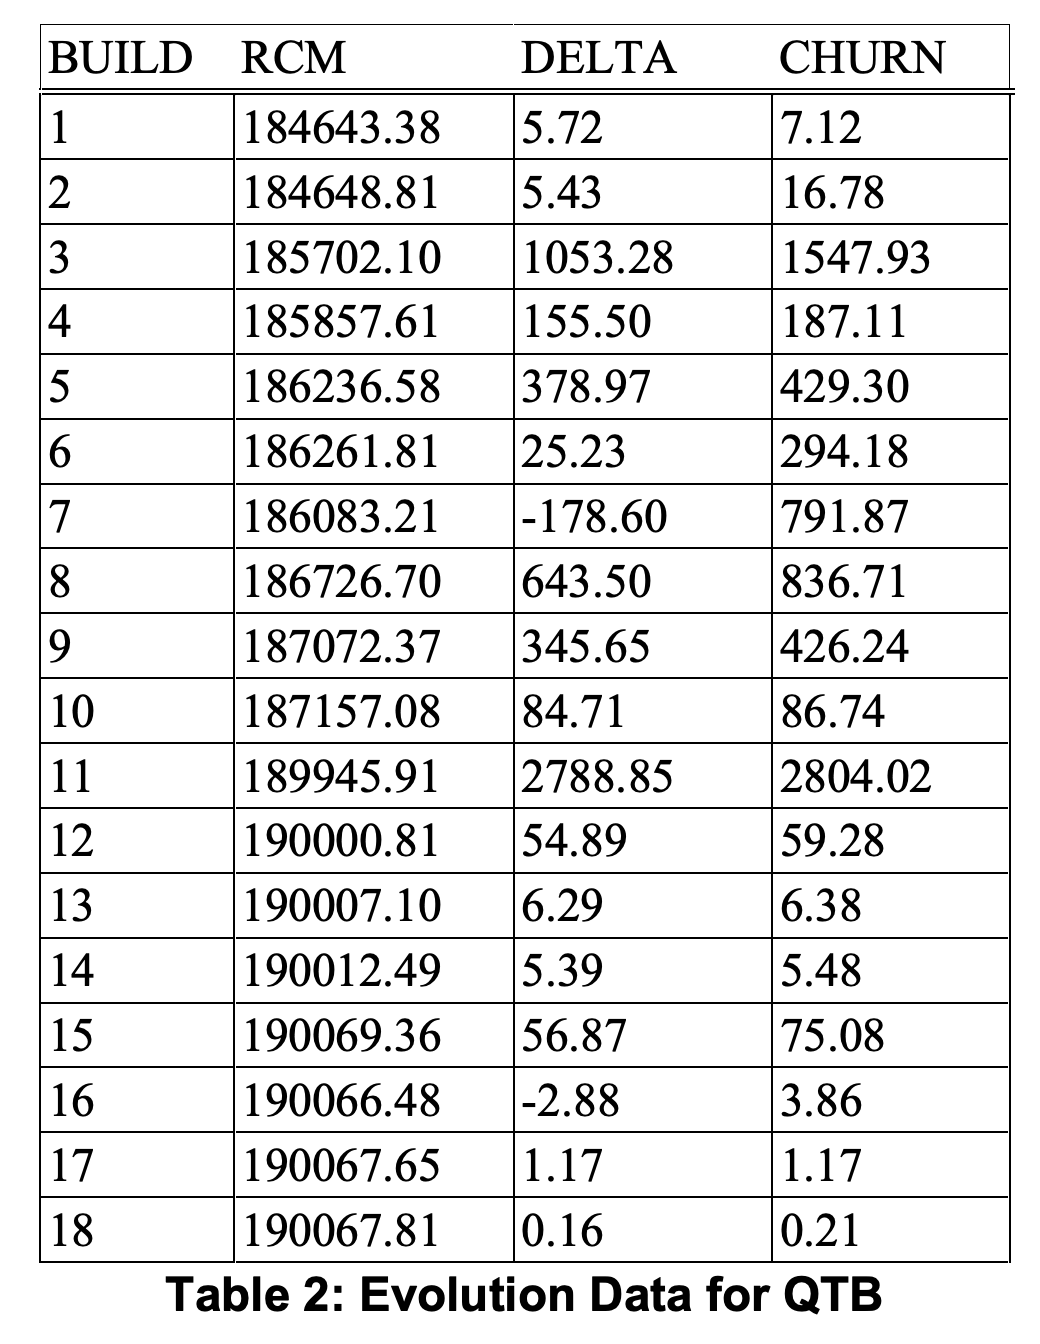
\includegraphics[width=.7\columnwidth]{qtb.png}
  \par\columnbreak\par
  ``A limitation of measuring \textcolor{orange}{code deltas} is that it
  \ul{doesn't} give an indicator as to how much change the
  system has undergone. If several
  software modules are removed and are replaced by
  modules of roughly equivalent complexity, the code
  delta for the system will be close to zero.''
  \par
  \lnSource{munson1998}
  \end{multicols}}

\lnPitch{
  \begin{multicols}{2}
  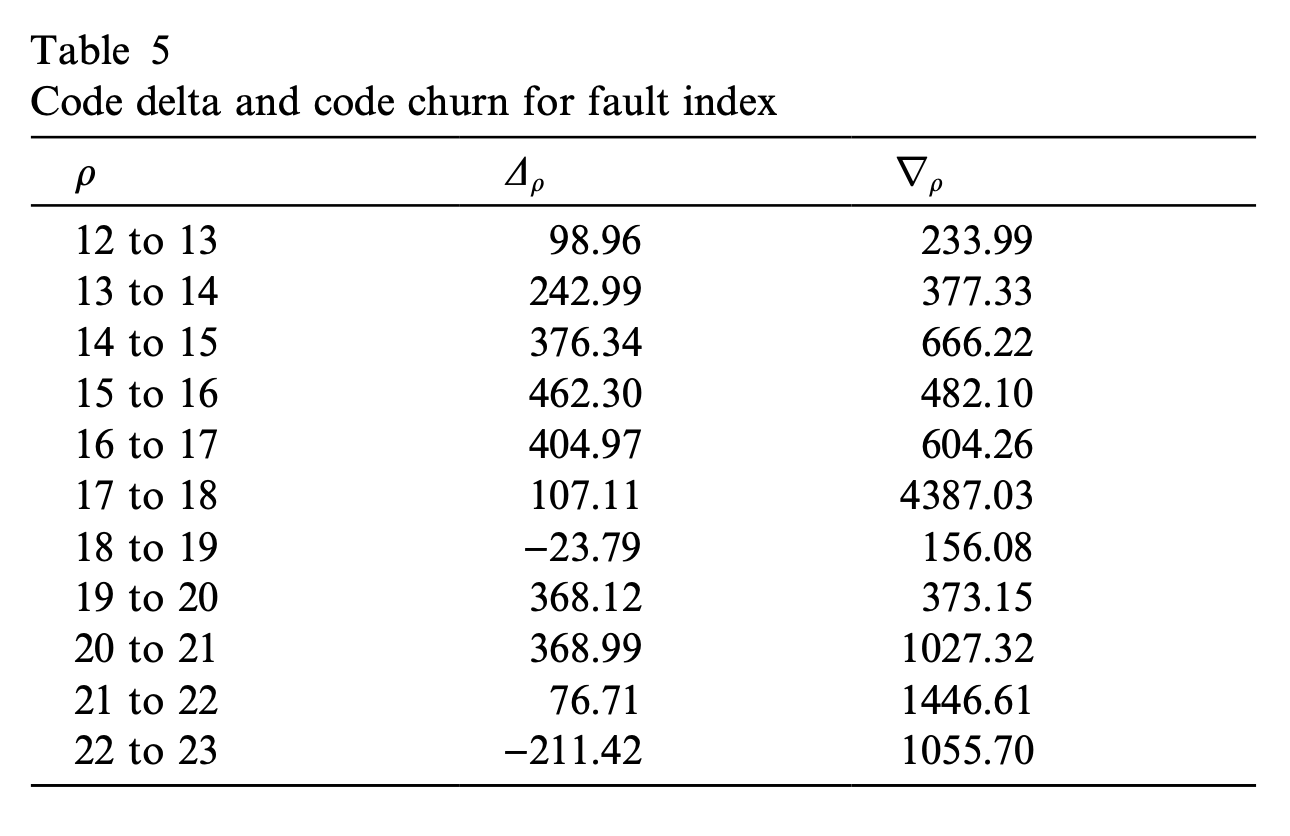
\includegraphics[width=\columnwidth]{fi-churn.png}
  \par\columnbreak\par
  ``In the case of code churn, what is important is the absolute measure of the amount of code that has been modified. From the standpoint of \ul{fault insertion} (FI), removing a lot of code is probably as catastrophic as adding a similar amount.''
  \par
  \lnSource{hall2000software}
  \end{multicols}}

\lnQuote
  [Nachiappan Nagappan]
  {nachiappan-nagappan}
  {Our case study provides strong support for the following conclusion: increase in relative code churn measures is accompanied by an increase in system \ul{defect density}.}
  {nagappan2005use}

\lnQuote
  [Rudolf Ferenc]
  {rudolf-ferenc}
  {We can conclude that committing files with higher cumulative code churn values (i.e. those of longer change history) is more likely to result in negative maintainability change.}
  {farago2015cumulative}

\lnQuote
[Tobias Olsson]
  {tobias-olsson}
  {Non-normal code churn can be a tangible and measurable \ul{effect} of architectural violations in source code. However, more research is needed to better understand this connection, e.g., if violations are the \ul{cause}, the size of the effect, the cost of refactoring, and whether it is generalizable to other system.}
  {olsson2017}

\lnPitch{
  \pptBanner{CodeClimate.com Interpretation of Code Churn}
  \begin{multicols}{2}
  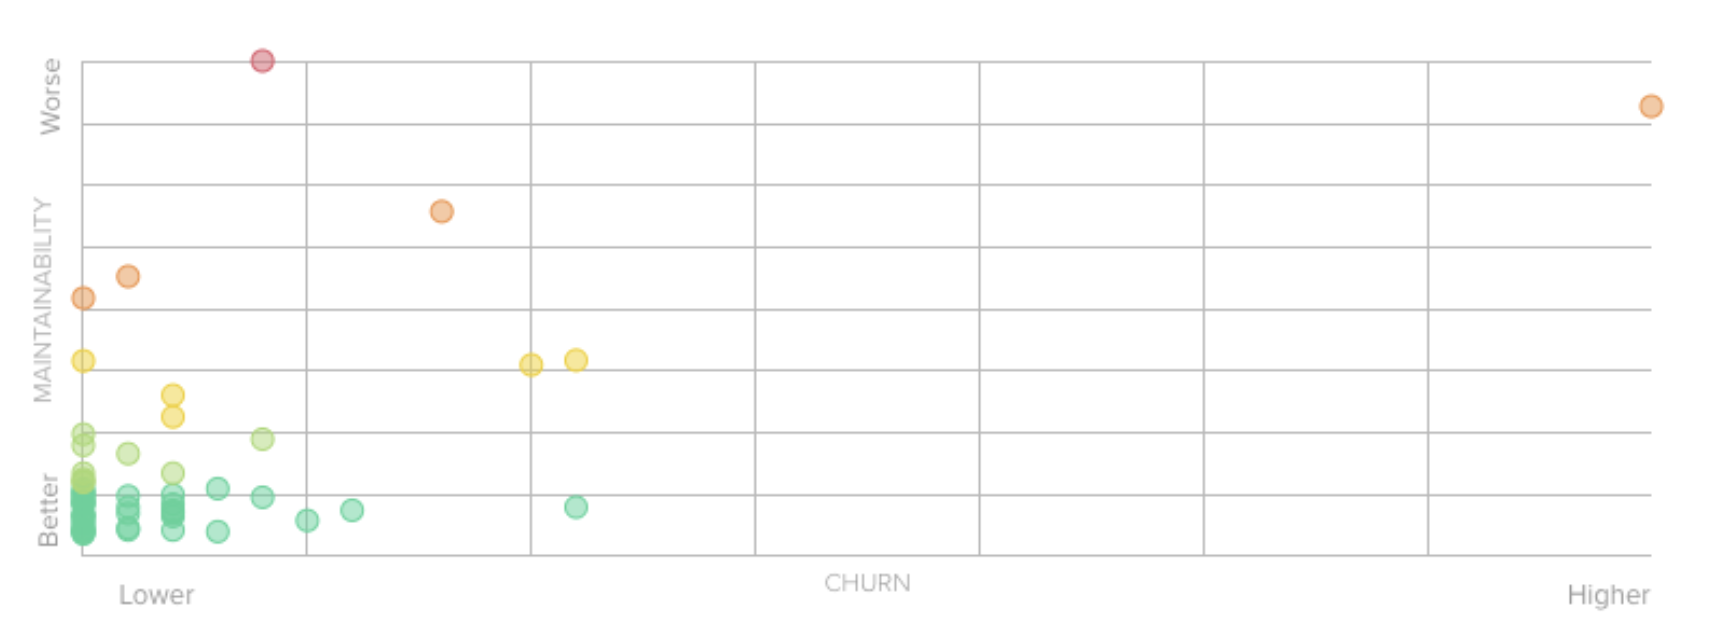
\includegraphics[width=.98\columnwidth]{codeclimate.png}
  \par\columnbreak\par
  ``When we have finished analyzing your default branch, you will see churn metrics for the files in your repository. This churn metric is approximately the \ul{number of times a file has changed} in the last 90 days, calculated by counting the number of distinct versions of that file across commits from that time.''\par
  {\scriptsize Source: \href{https://docs.codeclimate.com/docs/churn}{their blog}\par}
  \end{multicols}}

\lnPitch{
  \pptBanner{HitsOfCode.com}
  \begin{multicols}{2}
  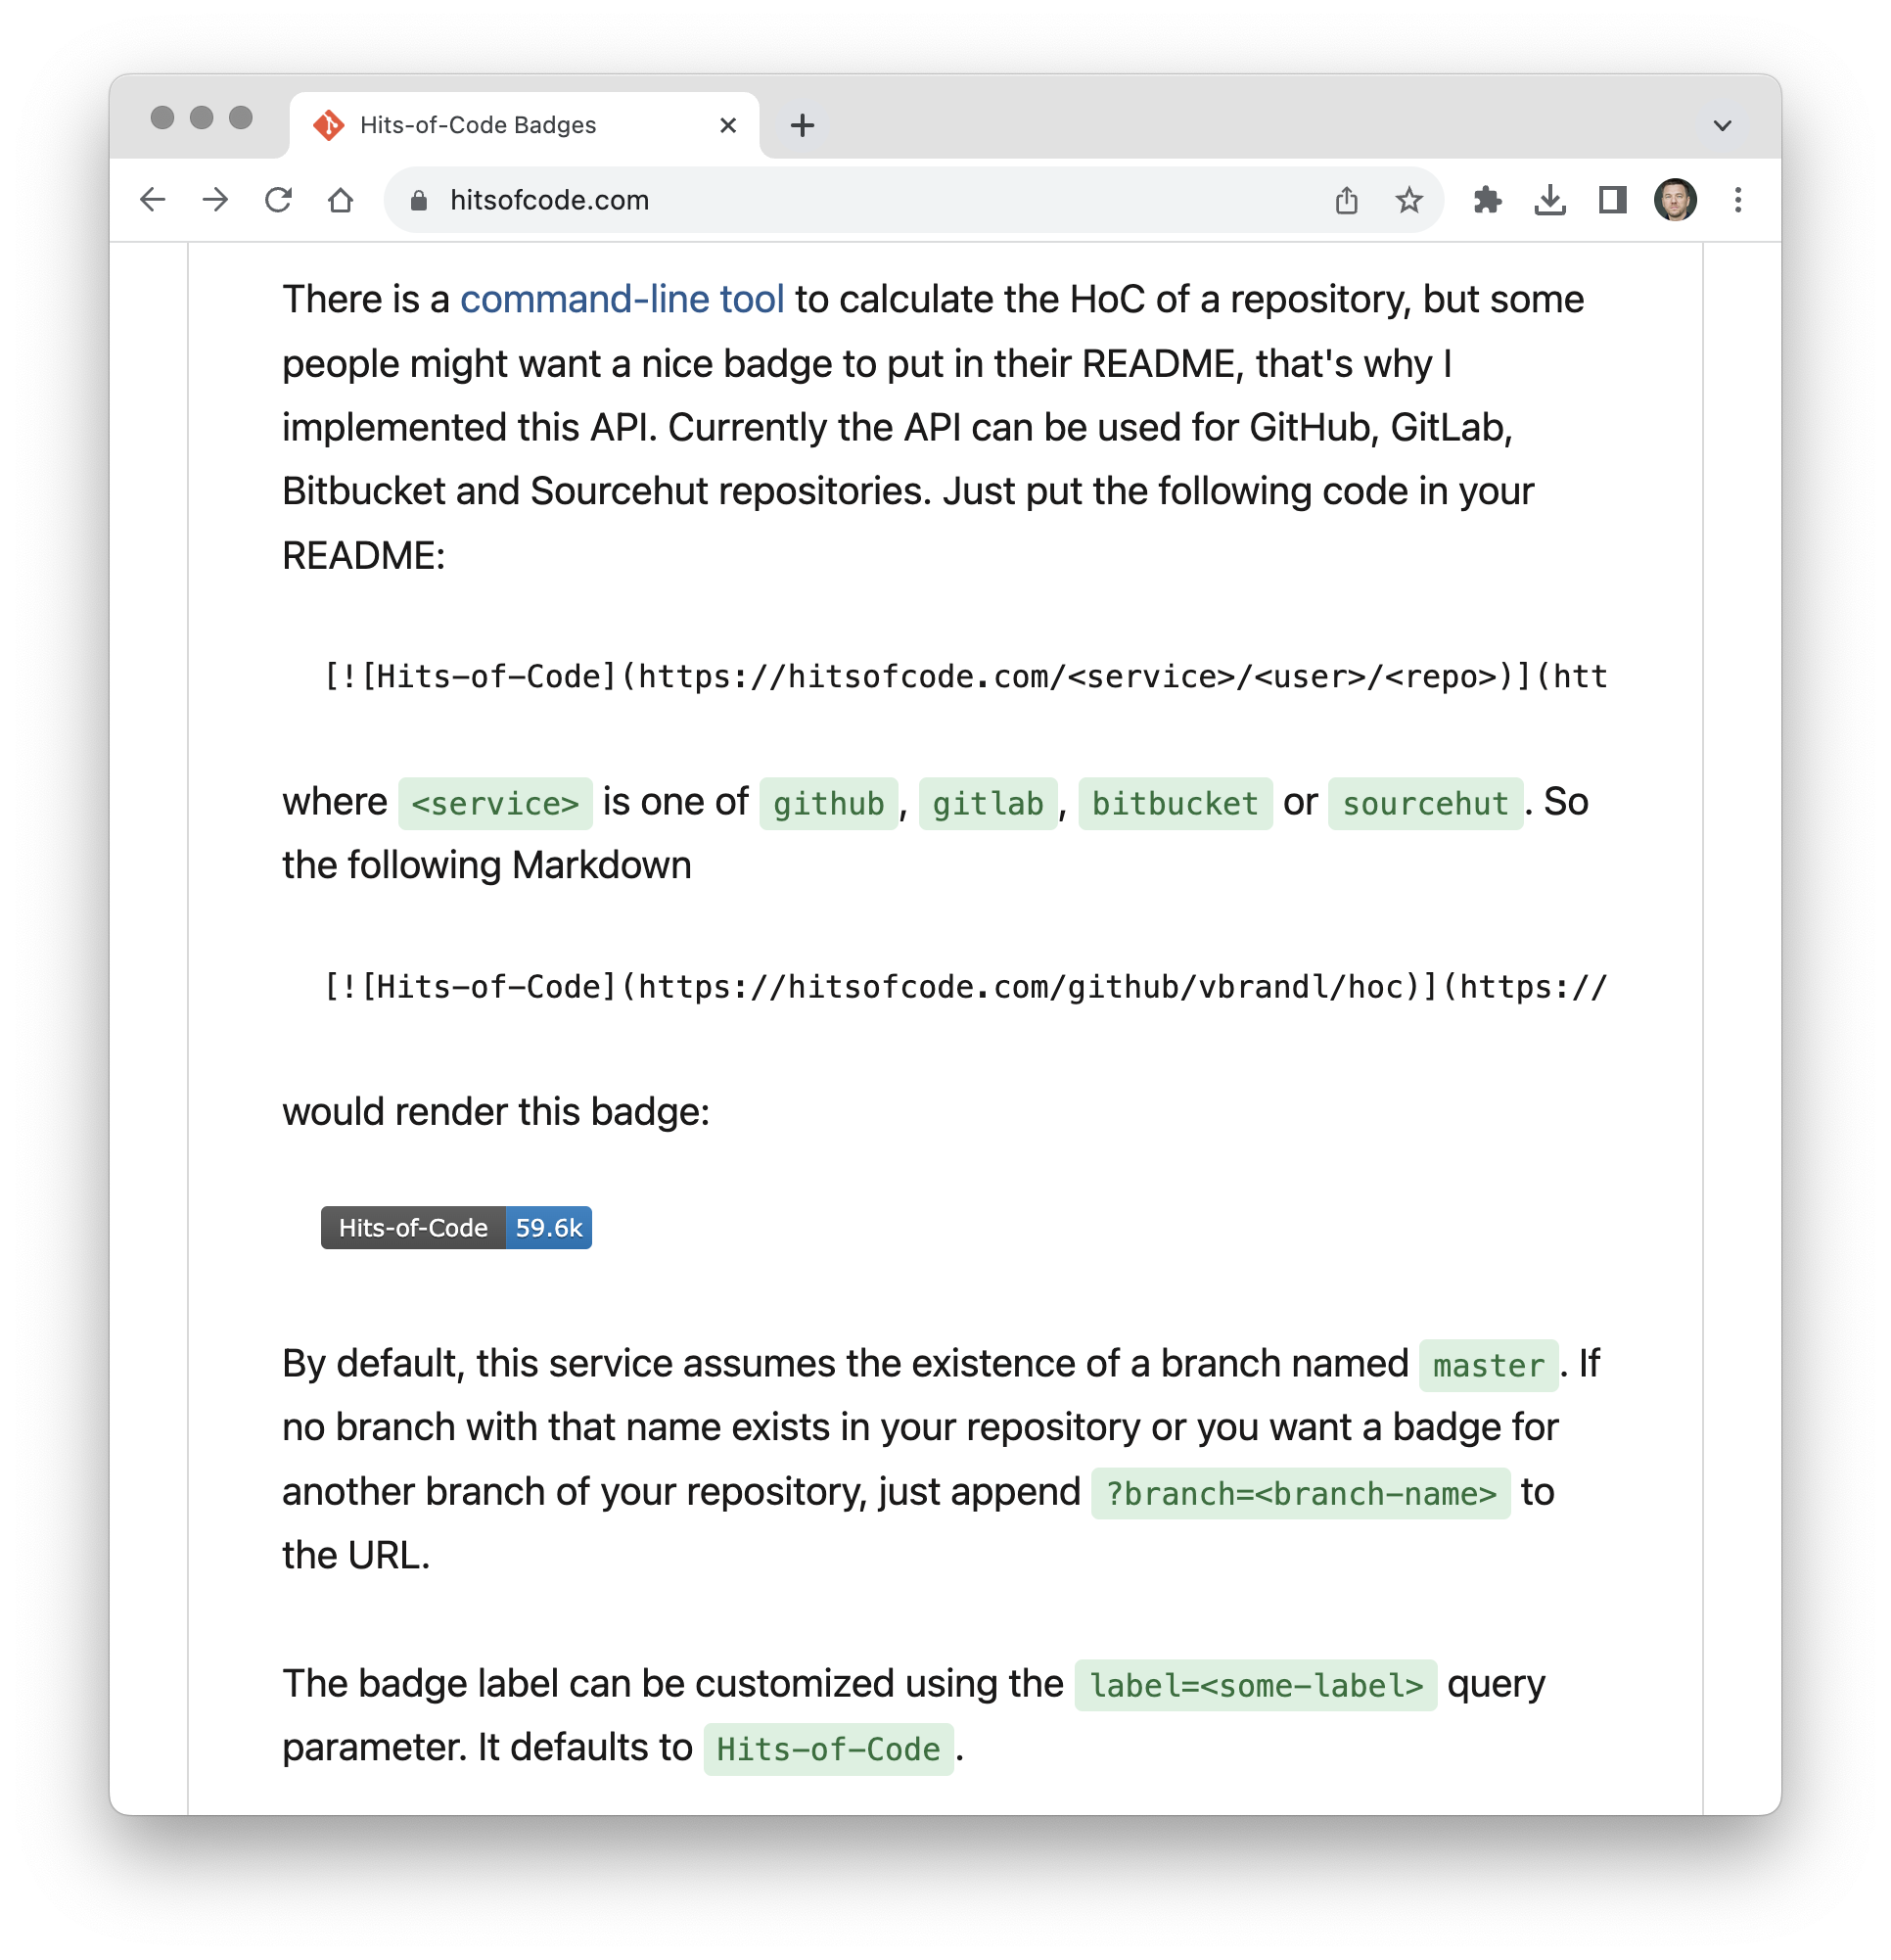
\includegraphics[width=.9\columnwidth]{hitsofcode.png}
  \par\columnbreak\par
  Created by \href{https://www.vbrandl.net/}{Valentin Brandl} (\href{https://github.com/vbrandl}{@vbrandl})
  and inspired by the blog post of mine~\citep{bugayenko2014blog1114}.
  \end{multicols}}

\end{document}
